\documentclass{beamer}
\usepackage[utf8]{inputenc}
\usepackage{graphicx, epsfig}
\usepackage{amsmath,mathrsfs,amsfonts,amssymb}
%\usepackage{subfig}
\usepackage{floatflt}
\usepackage{epic,ecltree}
\usepackage{mathtext}
\usepackage{fancybox}
\usepackage{fancyhdr}
\usepackage{multirow}
\usepackage{enumerate}
\usepackage{epstopdf}
\usepackage{multicol}
\usepackage{algorithm}
\usepackage[noend]{algorithmic}
\usepackage{tikz}
\usepackage{blindtext}
\usetheme{default}%{Singapore}%{Warsaw}%{Warsaw}%{Darmstadt}
\usecolortheme{default}
\setbeamerfont{title}{size=\Huge}
\setbeamertemplate{footline}[page number]{}


\makeatletter
\newcommand\HUGE{\@setfontsize\Huge{35}{40}}
\makeatother    

\setbeamerfont{title}{size=\HUGE}
\beamertemplatenavigationsymbolsempty

% latin bold lower
\newcommand{\ba}{\mathbf{a}} 
\newcommand{\bc}{\mathbf{c}} 
\newcommand{\be}{\mathbf{e}} 
\newcommand{\bh}{\mathbf{h}} 
\newcommand{\bp}{\mathbf{p}} 
\newcommand{\bt}{\mathbf{t}} 
\newcommand{\bs}{\mathbf{s}} 
\newcommand{\bu}{\mathbf{u}} 
\newcommand{\bv}{\mathbf{v}} 
\newcommand{\bw}{\mathbf{w}} 
\newcommand{\bx}{\mathbf{x}} 
\newcommand{\by}{\mathbf{y}} 
\newcommand{\bz}{\mathbf{z}} 

% latin bold upper
\newcommand{\bA}{\mathbf{A}} 
\newcommand{\bB}{\mathbf{B}} 
\newcommand{\bC}{\mathbf{C}} 
\newcommand{\bI}{\mathbf{I}} 
\newcommand{\bL}{\mathbf{L}} 
\newcommand{\bM}{\mathbf{M}} 
\newcommand{\bQ}{\mathbf{Q}} 
\newcommand{\bT}{\mathbf{T}} 
\newcommand{\bU}{\mathbf{U}} 
\newcommand{\bV}{\mathbf{V}} 
\newcommand{\bW}{\mathbf{W}} 
\newcommand{\bX}{\mathbf{X}} 
\newcommand{\bY}{\mathbf{Y}} 
\newcommand{\bZ}{\mathbf{Z}} 

% latin cal upper
\newcommand{\cG}{\mathcal{G}} 
\newcommand{\cL}{\mathcal{L}} 
\newcommand{\cN}{\mathcal{N}} 
\newcommand{\cS}{\mathcal{S}} 
\newcommand{\cT}{\mathcal{T}} 
\newcommand{\cW}{\mathcal{W}} 
\newcommand{\cX}{\mathcal{X}} 
\newcommand{\cZ}{\mathcal{Z}} 

% latin bb upper
\newcommand{\bbE}{\mathbb{E}} 
\newcommand{\bbI}{\mathbb{I}} 
\newcommand{\bbP}{\mathbb{P}} 
\newcommand{\bbR}{\mathbb{R}} 

% greek bold lower
\newcommand{\bepsilon}{\boldsymbol{\epsilon}} 
\newcommand{\btheta}{\boldsymbol{\theta}} 
\newcommand{\blambda}{\boldsymbol{\lambda}} 
\newcommand{\bpi}{\boldsymbol{\pi}} 
\newcommand{\bmu}{\boldsymbol{\mu}} 
\newcommand{\bsigma}{\boldsymbol{\sigma}} 
\newcommand{\bphi}{\boldsymbol{\phi}} 

% greek bold upper
\newcommand{\bSigma}{\boldsymbol{\Sigma}} 

\DeclareMathOperator*{\argmin}{arg\,min}
\DeclareMathOperator*{\argmax}{arg\,max}

\newcommand{\createdgmtitle}[1]{\title[\hbox to 56mm{Deep Generative Models  \hfill\insertframenumber\,/\,\inserttotalframenumber}]
	{\vspace{1.5cm} \\ Deep Generative Models \\ {\Huge Lecture #1}}
	\author{Roman Isachenko}
	\institute{
	Moscow Institute of Physics and Technology
	} 
	\date{Autumn, 2021}
}

\newcommand\myfootnote[1]{%
  \tikz[remember picture,overlay]
  \draw (current page.south west) +(1in + \oddsidemargin,0.5em)
  node[anchor=south west,inner sep=0pt]{\parbox{\textwidth}{%
      \rlap{\rule{10em}{0.4pt}}\raggedright\scriptsize \textit{#1}}};}

\newcommand\myfootnotewithlink[2]{%
  \tikz[remember picture,overlay]
  \draw (current page.south west) +(1in + \oddsidemargin,0.5em)
  node[anchor=south west,inner sep=0pt]{\parbox{\textwidth}{%
      \rlap{\rule{10em}{0.4pt}}\raggedright\scriptsize\href{#1}{\textit{#2}}}};}
\createdgmtitle{13}
%--------------------------------------------------------------------------------
\begin{document}
%--------------------------------------------------------------------------------
\begin{frame}[noframenumbering,plain]
%\thispagestyle{empty}
\titlepage
\end{frame}
%=======
\begin{frame}{Recap of previous lecture}
		\begin{itemize}
			\item $\cS_{\pi} = \{\bx_i\}_{i=1}^{n} \sim \pi(\bx)$ -- real samples;
			\item $\cS_{p} = \{\bx_i\}_{i=1}^{n} \sim p(\bx | \btheta)$ -- generated samples.
		\end{itemize}
		Embed samples using pretrained classifier network (as previously):
		\[
			\cG_{\pi} = \{\mathbf{g}_i\}_{i=1}^n, \quad \cG_{p} = \{\mathbf{g}_i\}_{i=1}^n.
		\]
		Define binary function:
		\[
			f(\mathbf{g}, \cG) = 
			\begin{cases}
				1, \text{if exists } \mathbf{g}' \in \cG: \| \mathbf{g}  - \mathbf{g}'\|_2 \leq \| \mathbf{g}' - \text{NN}_k(\mathbf{g}', \cG)\|_2; \\
				0, \text{otherwise.}
			\end{cases}
		\]
		\[
			\text{Precision} (\cG_{\pi}, \cG_{p}) = \frac{1}{n} \sum_{\mathbf{g} \in \cG_{p}} f(\mathbf{g}, \cG_{\pi}); \quad \text{Recall} (\cG_{\pi}, \cG_{p}) = \frac{1}{n} \sum_{\mathbf{g} \in \cG_{\pi}} f(\mathbf{g}, \cG_{p}).
		\]
		\vspace{-0.4cm}
		\begin{figure}
			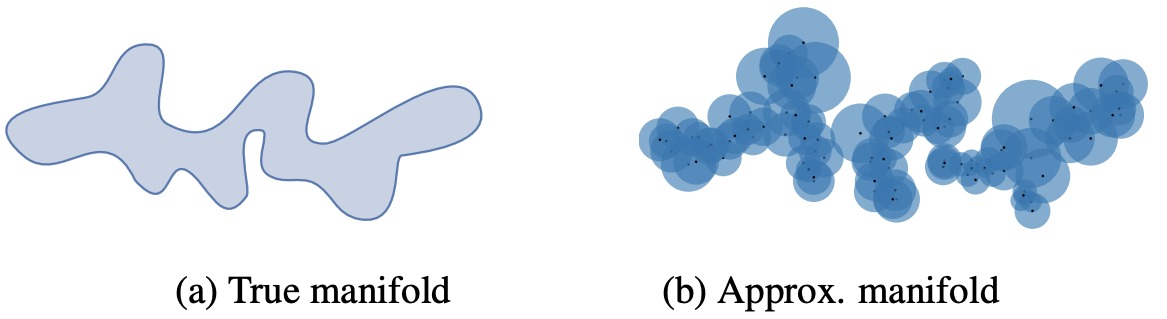
\includegraphics[width=0.7\linewidth]{figs/pr_k_nearest}
		\end{figure}
		\myfootnotewithlink{https://arxiv.org/abs/1904.06991}{Kynkäänniemi T. et al. Improved precision and recall metric for assessing generative models, 2019}
\end{frame}
%=======
\begin{frame}{Recap of previous lecture}
	\begin{figure}
		\centering
		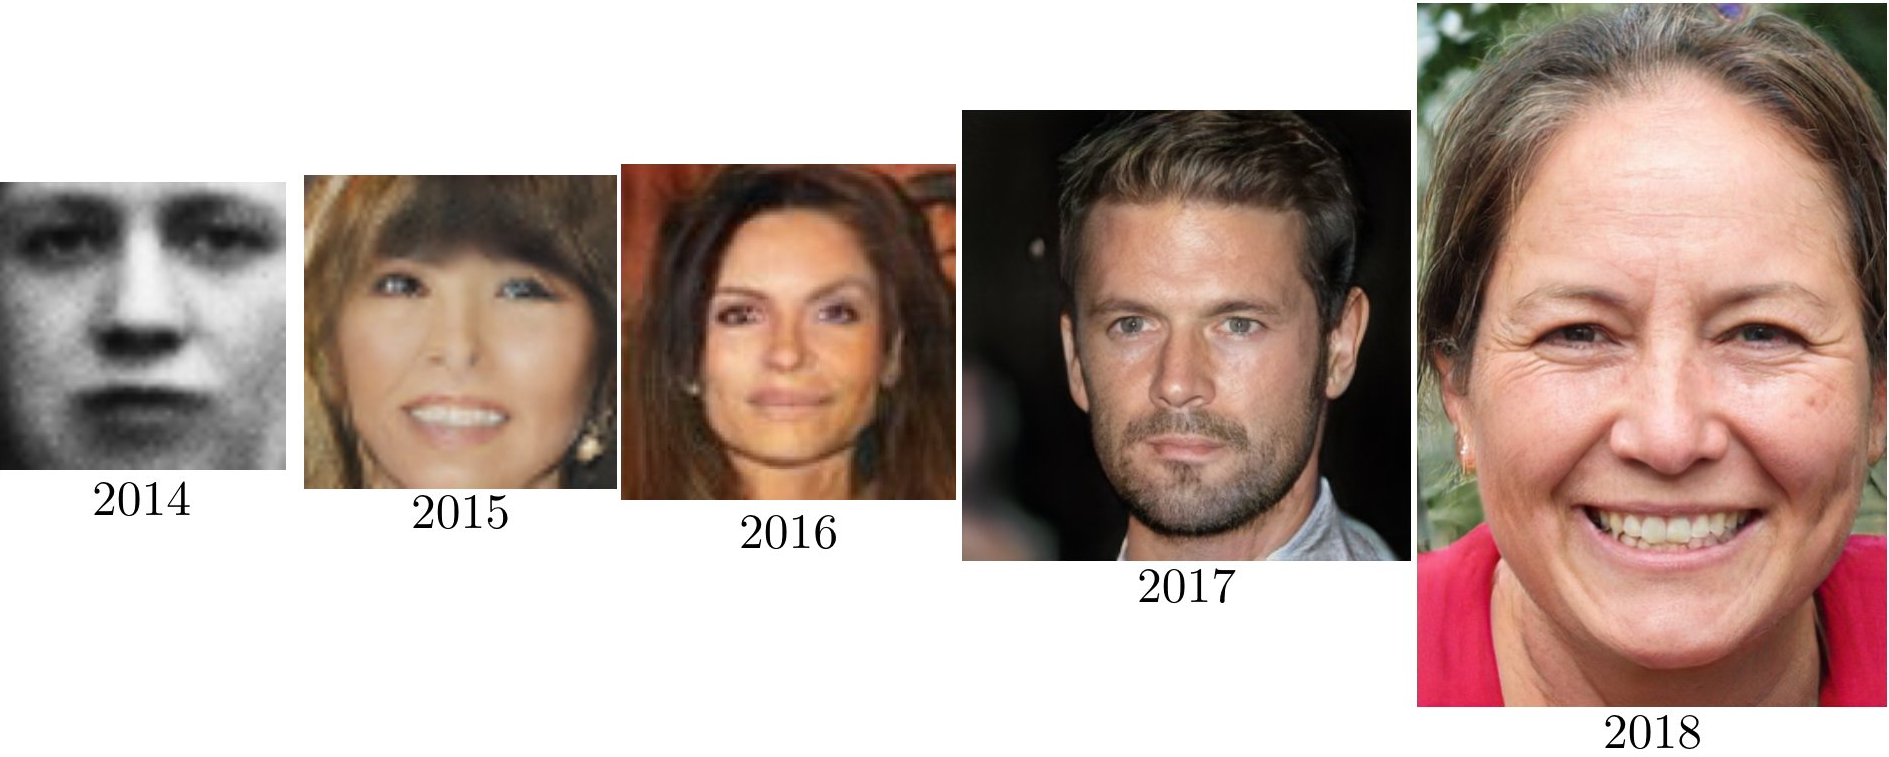
\includegraphics[width=\linewidth]{figs/gan_evolution}
	\end{figure}
	\begin{itemize}
		\item \textbf{Self-Attention GAN} allows to make huge receptive field and reduce convolution inductive bias.
		\item \textbf{BigGAN} shows that large batch size increase model quality gradually.
		\item \textbf{Progressive Growing GAN} starts from a low resolution, adds new layers that model fine details as training progresses.
		\item \textbf{StyleGAN}  introduces mapping network to get more disentangled latent representation.
	\end{itemize}
\end{frame}
%=======
\begin{frame}{Recap of previous lecture}
	\begin{block}{ELBO objective}
		\vspace{-0.5cm}
		\[
			 \mathcal{L} (\bphi, \btheta)  = \mathbb{E}_{q(\bz | \bx, \bphi)} \left[\log p(\bx | \bz, \btheta) + \log p(\bz) - \log q(\bz| \bx, \bphi) \right] \rightarrow \max_{\bphi, \btheta}.
		\]	
		\vspace{-0.5cm}
	\end{block}
	What is the problem to make the variational posterior model an \textbf{implicit} model? \\
	 We have to estimate density ratio 
	\[
		r(\bx, \bz) = \frac{q_1(\bx, \bz)}{q_2(\bx, \bz)} = \frac{p(\bz) \pi(\bx)}{q(\bz| \bx, \bphi) \pi (\bx)}.
	\] 
	\begin{block}{Adversarial Variational Bayes}
		\vspace{-0.6cm}
		\[
			\max_D \left[ \bbE_{\pi(\bx)} \bbE_{q(\bz | \bx, \bphi)} \log D(\bx, \bz) + \bbE_{\pi(\bx)} \bbE_{p(\bz)} \log (1 - D(\bx, \bz)) \right]
		\]
	\end{block}
	\myfootnotewithlink{https://arxiv.org/abs/1701.04722}{Mescheder L., Nowozin S., Geiger A. Adversarial variational bayes: Unifying variational autoencoders and generative adversarial networks, 2017}
\end{frame}
%=======
\begin{frame}{Neural ODE}
	Consider Ordinary Differential Equation    
	\begin{align*}
	    \frac{d \bz(t)}{dt} &= f(\bz(t), \btheta); \quad \text{with initial condition }\bz(t_0) = \bz_0. \\
	    \bz(t_1) &= \int^{t_1}_{t_0} f(\bz(t), \btheta) d t  + \bz_0 = \text{ODESolve}(\bz(t_0), f, t_0,t_1, \btheta).
	\end{align*}
	\vspace{-0.4cm}
	\begin{block}{Euler update step}
		\vspace{-0.6cm}
		\[
		    \frac{\bz(t + \Delta t) - \bz(t)}{\Delta t} = f(\bz(t), \btheta) \quad \Rightarrow \quad \bz(t + \Delta t) = \bz(t) + \Delta t f(\bz(t), \btheta).
		\]
		\vspace{-0.7cm}
	\end{block}
	\begin{block}{Residual block}
		\begin{minipage}[t]{0.7\columnwidth}
			\vspace{-0.4cm}
			\[
				\bz_{t + 1} = \bz_t + f(\bz_t, \btheta)
			\]
			\vspace{-0.6cm}
			\begin{itemize}
				 \item It is equavalent to Euler update step for solving ODE with $\Delta t = 1$!
				 \item Euler update step is unstable and trivial. There are more sophisticated methods.
			\end{itemize}
		\end{minipage}%
		\begin{minipage}[t]{0.3\columnwidth}
			\vspace{-0.2cm}
			\begin{figure}
			    \centering
			    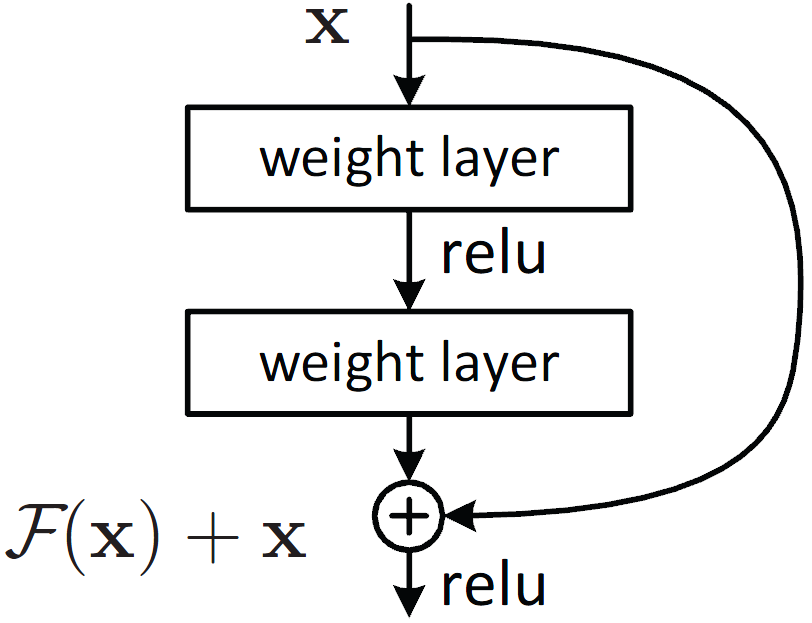
\includegraphics[width=\linewidth]{figs/resnet_1.png}
			\end{figure}
		\end{minipage}
		\vspace{-0.4cm}
	\end{block}

	\myfootnotewithlink{https://arxiv.org/abs/1806.07366}{Chen R. T. Q. et al. Neural Ordinary Differential Equations, 2018}   
\end{frame}
%=======
\begin{frame}{Neural ODE}
	\begin{block}{Residual block}
	\vspace{-0.4cm}
	\[
	    \bz_{t+1} = \bz_t + f(\bz_t, \btheta).
	\]
	\vspace{-0.4cm}
	\end{block}
	In the limit of adding more layers and taking smaller steps, we parameterize the continuous dynamics of hidden units using an ODE specified by a neural network: 
	\[
	    \frac{d \bz(t)}{dt} = f(\bz(t), t, \btheta); \quad \bz(t_0) = \bx; \quad \bz(t_1) = \by.
	\]
	\begin{minipage}[t]{0.4\columnwidth}
		\begin{figure}
			\centering
			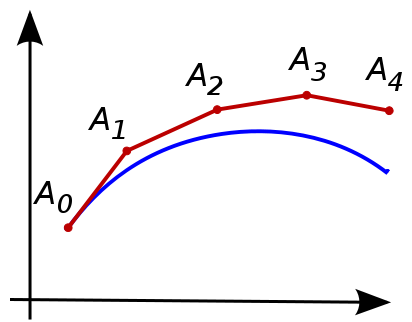
\includegraphics[width=0.8\linewidth]{figs/euler}
		\end{figure}
	\end{minipage}%
	\begin{minipage}[t]{0.6\columnwidth}
		\vspace{-0.4cm}
		\begin{figure}
			\centering
			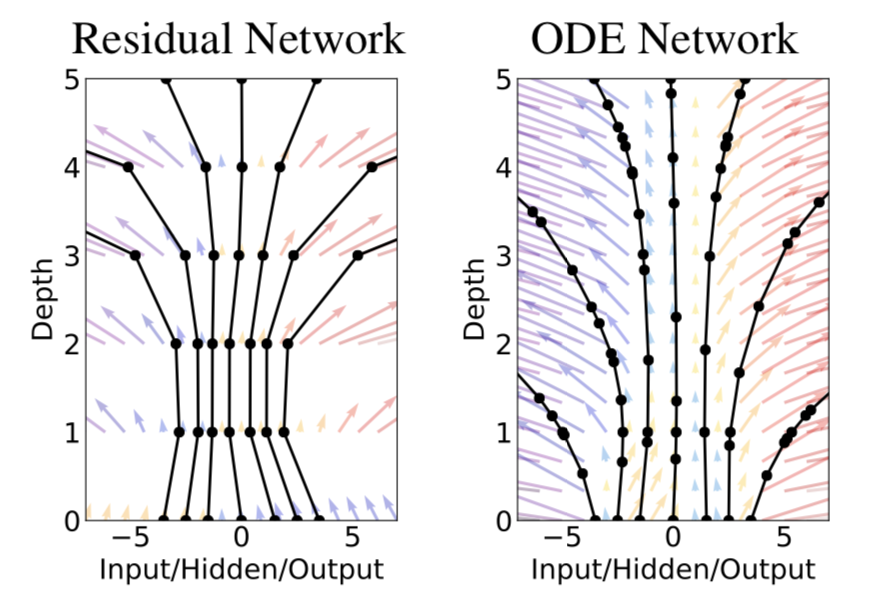
\includegraphics[width=0.9\linewidth]{figs/resnet_vs_neural_ode.png}
		\end{figure}
	\end{minipage}

	\myfootnotewithlink{https://arxiv.org/abs/1806.07366}{Chen R. T. Q. et al. Neural Ordinary Differential Equations, 2018}   
\end{frame}
%=======

\begin{frame}{Neural ODE}
	\begin{block}{Forward pass (loss function)}
		\vspace{-0.8cm}
		\begin{align*}
			L(\by) = L(\bz(t_1)) &= L\left( \bz(t_0) + \int_{t_0}^{t_1} f(\bz(t), \btheta) dt \right) \\ &= L\bigl(\text{ODESolve}(\bz(t_0), f, t_0,t_1, \btheta) \bigr)
		\end{align*}
	\vspace{-0.5cm}
	\end{block}
	\textbf{Note:} ODESolve could be any method (Euler step, Runge-Kutta methods).
	\begin{block}{Backward pass (gradients computation)}
		For fitting parameters we need gradients:
		\[
			\ba_{\bz}(t) = \frac{\partial L(\by)}{\partial \bz(t)}; \quad \ba_{\btheta}(t) = \frac{\partial L(\by)}{\partial \btheta(t)}.
		\]
		In theory of optimal control these functions called \textbf{adjoint} functions. 
		They show how the gradient of the loss depends on the hidden state~$\bz(t)$ and parameters $\btheta$.
	\end{block}

	\myfootnotewithlink{https://arxiv.org/abs/1806.07366}{Chen R. T. Q. et al. Neural Ordinary Differential Equations, 2018}     
\end{frame}
%=======
\begin{frame}{Neural ODE}
	\begin{block}{Adjoint functions}
		\vspace{-0.3cm}
		\[
			\ba_{\bz}(t) = \frac{\partial L(\by)}{\partial \bz(t)}; \quad \ba_{\btheta}(t) = \frac{\partial L(\by)}{\partial \btheta(t)}.
		\]
		\vspace{-0.6cm}
	\end{block}
	\begin{block}{Theorem (Pontryagin)}
	\vspace{-0.6cm}
	\[
	     \frac{d \ba_{\bz}(t)}{dt} = - \ba_{\bz}(t)^T \cdot \frac{\partial f(\bz(t), \btheta)}{\partial \bz}; \quad \frac{d \ba_{\btheta}(t)}{dt} = - \ba_{\bz}(t)^T \cdot \frac{\partial f(\bz(t), \btheta)}{\partial \btheta}.
	\]
	Do we know any initilal condition?
	\end{block}
	\begin{block}{Solution for adjoint function}
		\vspace{-0.8cm}
		\begin{align*}
			 \frac{\partial L}{\partial \btheta(t_0)} &= \ba_{\btheta}(t_0) =  - \int_{t_1}^{t_0} \ba_{\bz}(t)^T \frac{\partial f(\bz(t), \btheta)}{\partial \btheta(t)} dt + 0\\
			 \frac{\partial L}{\partial \bz(t_0)} &= \ba_{\bz}(t_0) =  - \int_{t_1}^{t_0} \ba_{\bz}(t)^T \frac{\partial f(\bz(t), \btheta)}{\partial \bz(t)} dt + \frac{\partial L}{\partial \bz(t_1)}\\
		\end{align*}
		\vspace{-1.5cm}
	\end{block}
	\textbf{Note:} These equations are solved back in time.
	\myfootnotewithlink{https://arxiv.org/abs/1806.07366}{Chen R. T. Q. et al. Neural Ordinary Differential Equations, 2018}   
\end{frame}
%=======
\begin{frame}{Neural ODE}
	\vspace{-0.2cm}
	\begin{block}{Forward pass}
		\vspace{-0.5cm}
		\[
			\bz(t_1) = \int^{t_1}_{t_0} f(\bz(t), \btheta) d t  + \bz_0 \quad \Rightarrow \quad \text{ODE Solver}
		\]
		\vspace{-0.6cm}
	\end{block}
	\begin{block}{Backward pass}
		\vspace{-0.8cm}
		\begin{equation*}
			\left.
				{\footnotesize 
				\begin{aligned}
					\frac{\partial L}{\partial \btheta(t_0)} &= \ba_{\btheta}(t_0) =  - \int_{t_1}^{t_0} \ba_{\bz}(t)^T \frac{\partial f(\bz(t), \btheta)}{\partial \btheta(t)} dt + 0 \\
					\frac{\partial L}{\partial \bz(t_0)} &= \ba_{\bz}(t_0) =  - \int_{t_1}^{t_0} \ba_{\bz}(t)^T \frac{\partial f(\bz(t), \btheta)}{\partial \bz(t)} dt + \frac{\partial L}{\partial \bz(t_1)} \\
					\bz(t_0) &= - \int^{t_0}_{t_1} f(\bz(t), \btheta) d t  + \bz_1.
				\end{aligned}
				}
			\right\rbrace
			 \Rightarrow
			\text{ODE Solver}
		\end{equation*}
		\vspace{-0.4cm} 
	\end{block}
	\textbf{Note:} These scary formulas are the standard backprop in the discrete case.
	\begin{figure}
		\centering
		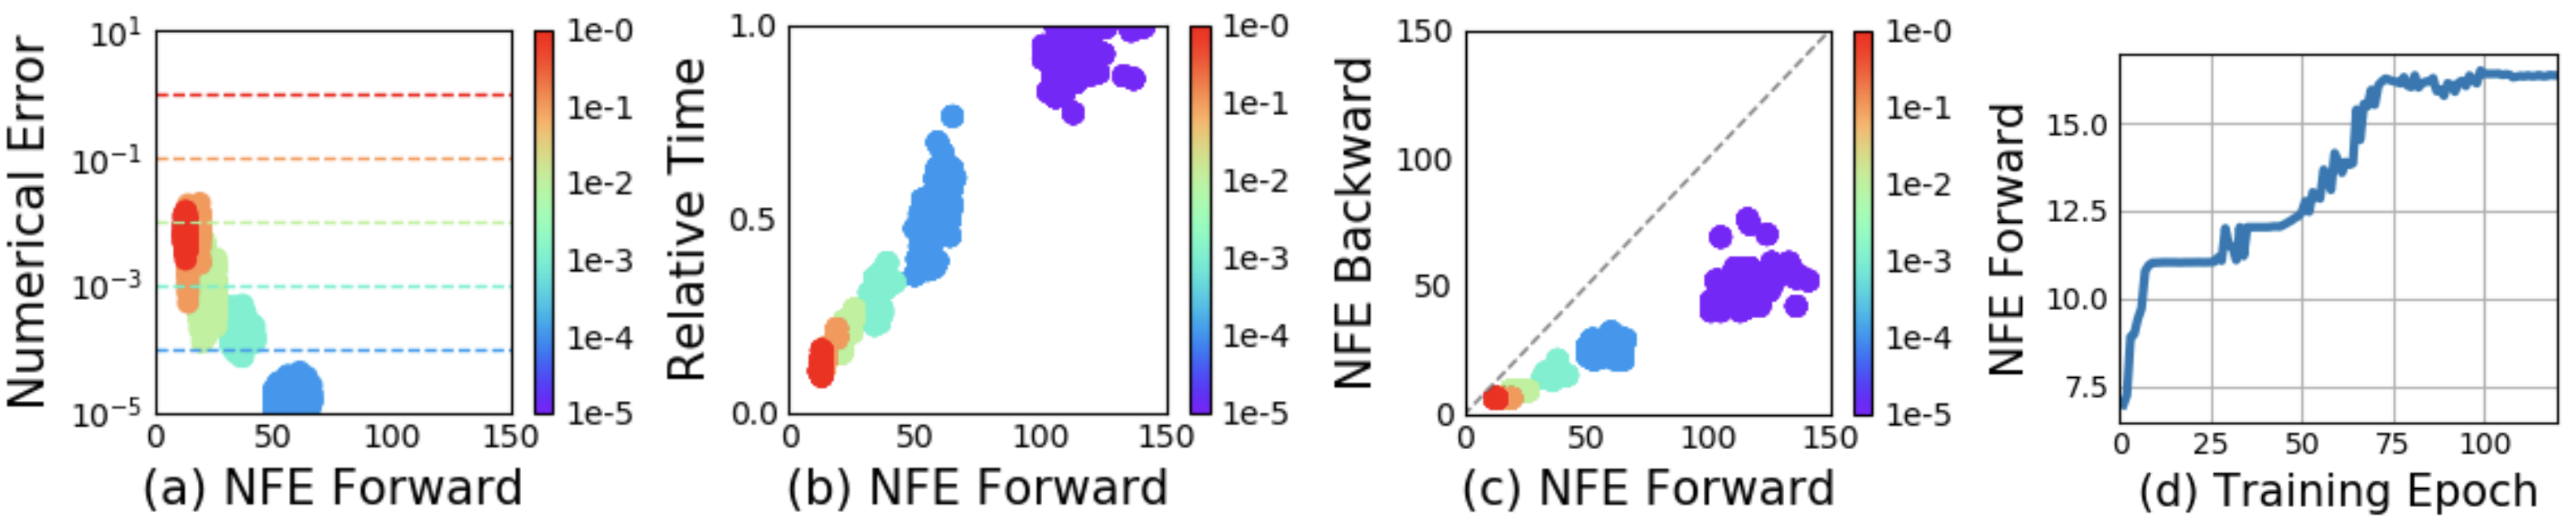
\includegraphics[width=\linewidth]{figs/neural_ode}
	\end{figure}
	\myfootnotewithlink{https://arxiv.org/abs/1806.07366}{Chen R. T. Q. et al. Neural Ordinary Differential Equations, 2018}   
\end{frame}
%=======
\begin{frame}{Continuous Normalizing Flows}
	\begin{block}{Discrete Normalizing Flows}
		\vspace{-0.8cm}
		  \[
		  \bz_{t+1} = f(\bz_t, \btheta); \quad \log p(\bz_{t+1}) = \log p(\bz_{t}) - \log \left| \det \frac{\partial f(\bz_t, \btheta)}{\partial \bz_{t}} \right| .
		  \]
		\vspace{-0.7cm}
	\end{block}
	\begin{block}{Continuous-in-time dynamic transformation}
		\vspace{-0.2cm}
		\[
			\frac{d\bz(t)}{dt} = f(\bz(t), \btheta).
		\]
		\vspace{-0.4cm}
	\end{block}
	Assume that function $f$ is uniformly Lipschitz continuous in $\bz$ and continuous in $t$. From Picard’s existence theorem, it follows that the above ODE has a \textbf{unique solution}.
	\begin{block}{Forward and inverse transforms}
		\vspace{-0.7cm}
		\begin{align*}
			\bx &= \bz(t_1) = \bz(t_0) + \int_{t_0}^{t_1} f(\bz(t), \btheta) dt \\
			\bz &= \bz(t_0) = \bz(t_1) + \int_{t_1}^{t_0} f(\bz(t), \btheta) dt \\
		\end{align*}
	\end{block}
	\myfootnotewithlink{https://arxiv.org/abs/1912.02762}{Papamakarios G. et al. Normalizing flows for probabilistic modeling and inference, 2019}   
\end{frame}
%=======
\begin{frame}{Continuous Normalizing Flows}
	To train this flow we have to get the way to calculate the density~$p(\bz(t))$.
	\begin{block}{Theorem (Fokker-Planck)}
		if function $f$ is uniformly Lipschitz continuous in $\bz$ and continuous in $t$, then
		\vspace{-0.3cm}
		\[
			\frac{\partial \log p(\bz(t))}{\partial t} = - \text{trace} \left( \frac{\partial f (\bz(t), \btheta)}{\partial \bz(t)} \right).
		\]
		\vspace{-0.5cm}
	\end{block}
	\textbf{Note:} Unlike discrete-in-time flows, the function $f$ does not need to be bijective, because uniqueness guarantees that the entire transformation is automatically bijective.
	\begin{block}{Density evaluation}
		\vspace{-0.4cm}
		\[
			\log p(\bx | \btheta) = \log p(\bz) - \int_{t_0}^{t_1} \text{trace}  \left( \frac{\partial f (\bz(t), \btheta)}{\partial \bz(t)} \right) dt.
		\]
		\textbf{Adjoint} method is used to integral evaluation.
	\end{block}
	\myfootnotewithlink{https://arxiv.org/abs/1806.07366}{Chen R. T. Q. et al. Neural Ordinary Differential Equations, 2018}   
\end{frame}
%=======
\begin{frame}{Continuous Normalizing Flows}
	\vspace{-0.6cm}
	\begin{block}{Forward transform + log-density}
		\vspace{-0.8cm}
		\[
			\begin{bmatrix}
				\bx \\
				\log p(\bx | \btheta)
			\end{bmatrix}
			= 
			\begin{bmatrix}
				\bz \\
				\log p(\bz)
			\end{bmatrix} + 
			\int_{t_0}^{t_1} 
			\begin{bmatrix}
				f(\bz(t), \btheta) \\
				- \text{trace} \left( \frac{\partial f(\bz(t), \btheta)}{\partial \bz(t)} \right) 
			\end{bmatrix} dt.
		\]
		\vspace{-0.6cm}
	\end{block}
	\begin{itemize}
		\item Discrete-in-time normalizing flows need invertible $f$. It costs $O(d^3)$ to get determinant of Jacobian.
		\item Continuous-in-time flows require only smoothness of $f$. It costs $O(d^2)$ to get trace of Jacobian.
	\end{itemize}
	\vspace{-0.5cm}
	\begin{minipage}[t]{0.4\columnwidth}
		\begin{figure}
			\centering
			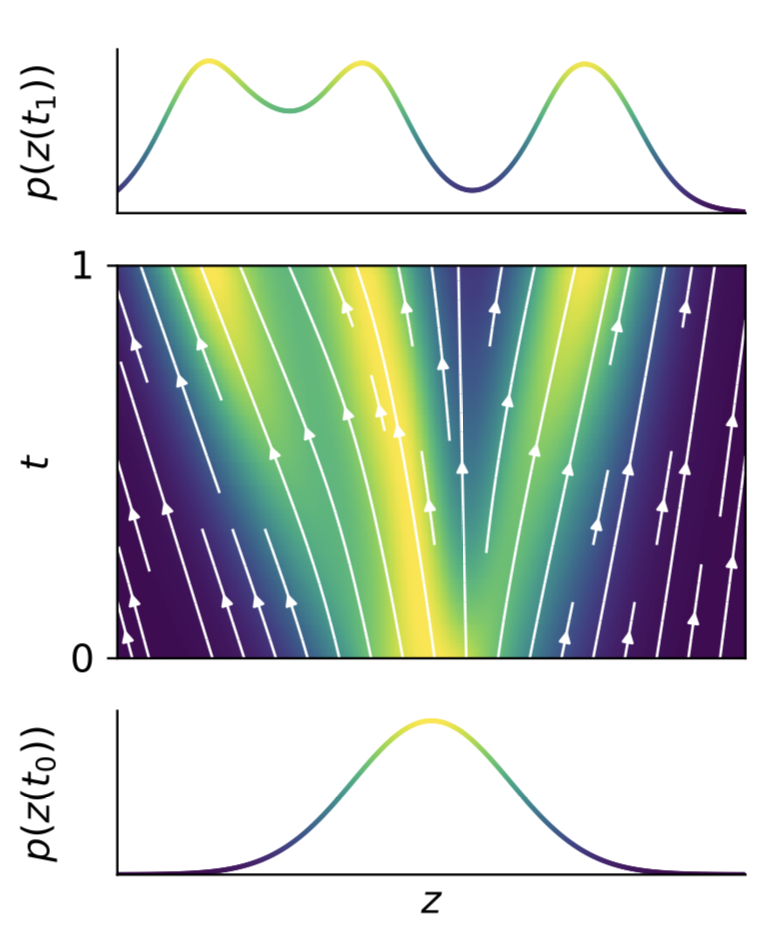
\includegraphics[width=0.75\linewidth]{figs/cnf_flow.png}
		\end{figure}
	\end{minipage}%
	\begin{minipage}[t]{0.6\columnwidth}
		\begin{figure}
			  \centering
			  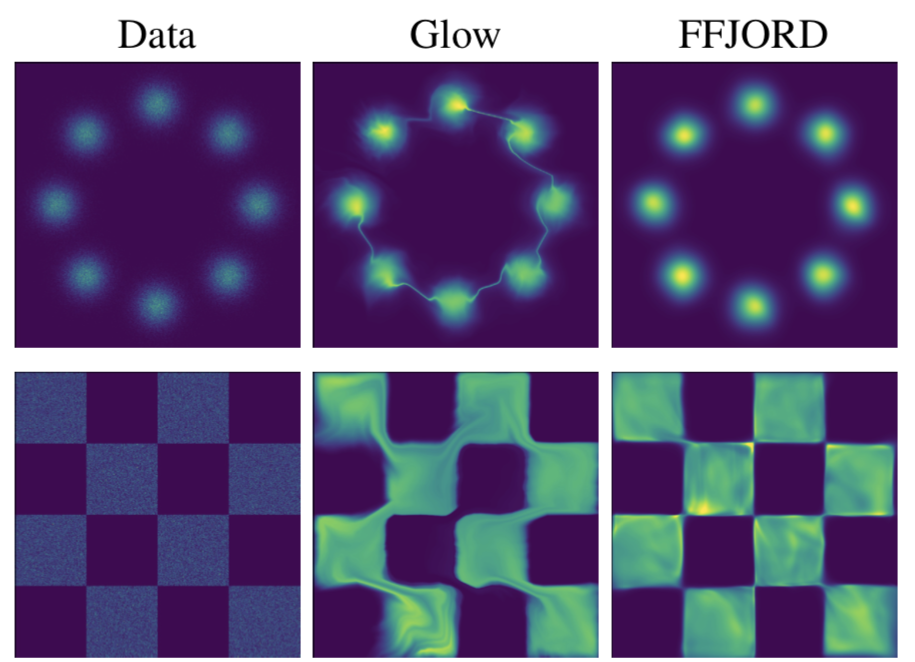
\includegraphics[width=0.8\linewidth]{figs/ffjord.png}
		\end{figure}
	\end{minipage}
	\myfootnotewithlink{https://arxiv.org/abs/1810.01367}{Grathwohl W. et al. FFJORD: Free-form Continuous Dynamics for Scalable Reversible Generative Models, 2018} 
\end{frame}
%=======
\begin{frame}{FFJORD}
	\begin{figure}
		\centering
		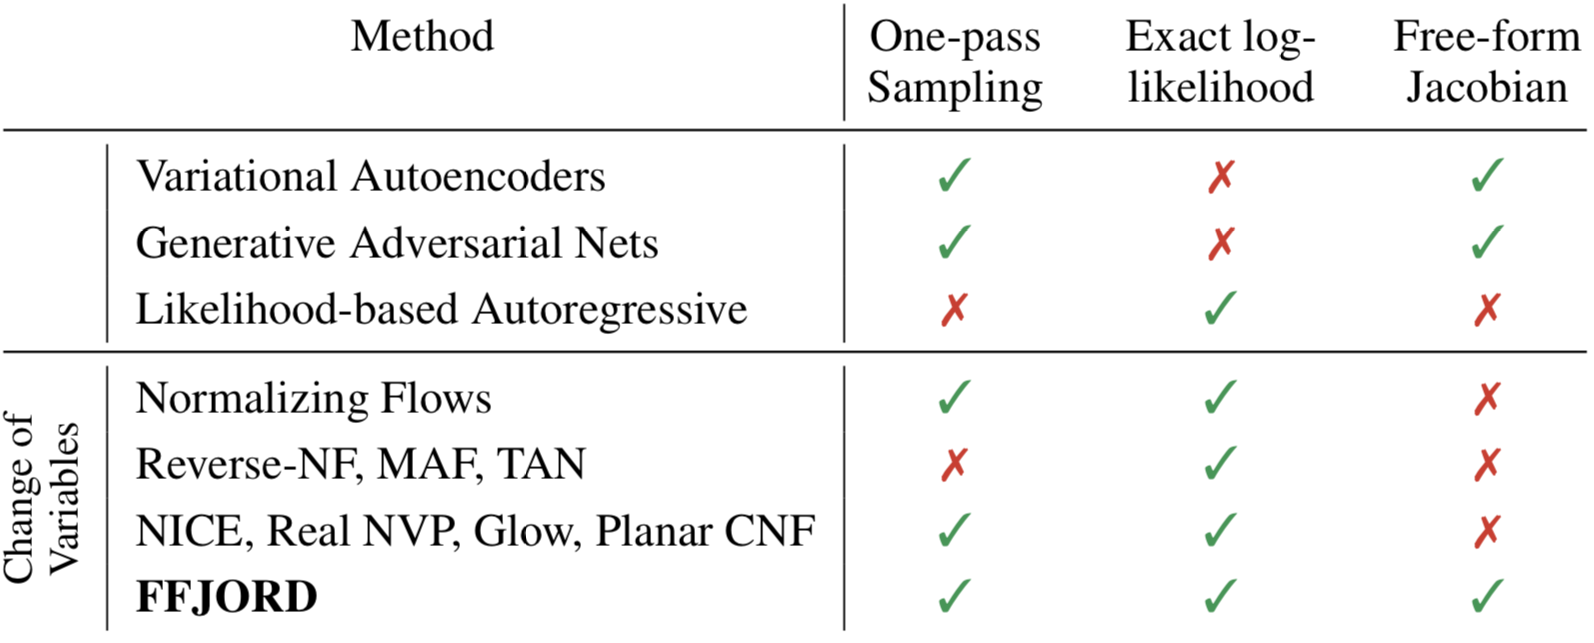
\includegraphics[width=0.75\linewidth]{figs/flow_comparison.png}
	\end{figure}
	\vspace{-0.4cm}
	\begin{block}{Density estimation (forward KL)}
		\vspace{-0.2cm}
		\begin{figure}
			\centering
			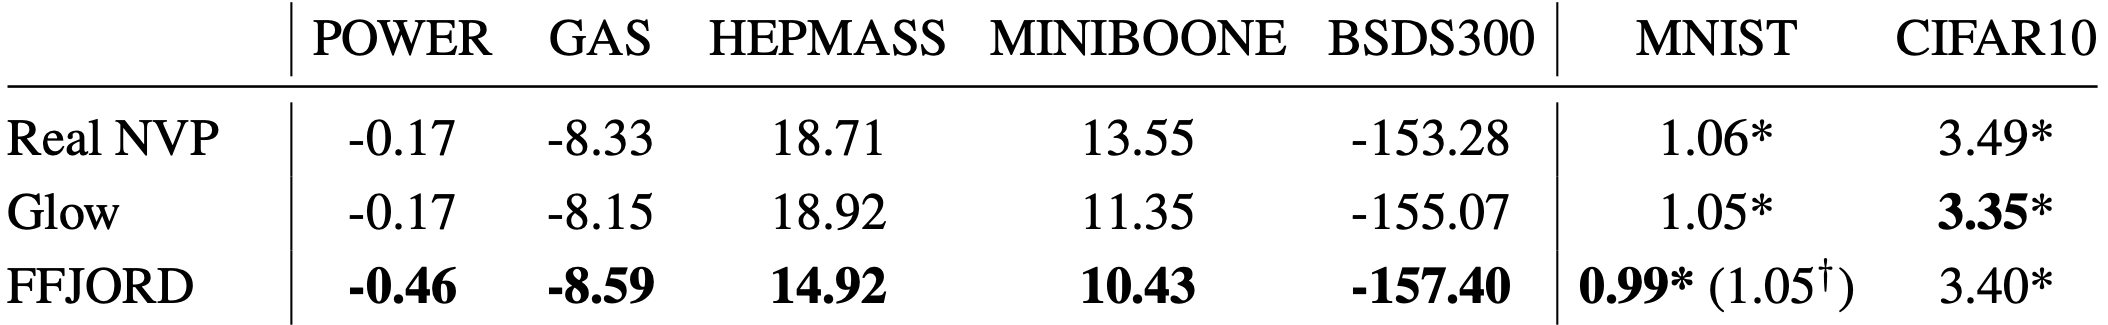
\includegraphics[width=0.8\linewidth]{figs/ffjord_forward}
		\end{figure}
		\vspace{-0.5cm}
	\end{block}
	\begin{block}{Flows for variational inference (reverse KL)}
		\vspace{-0.2cm}
		\begin{figure}
			\centering
			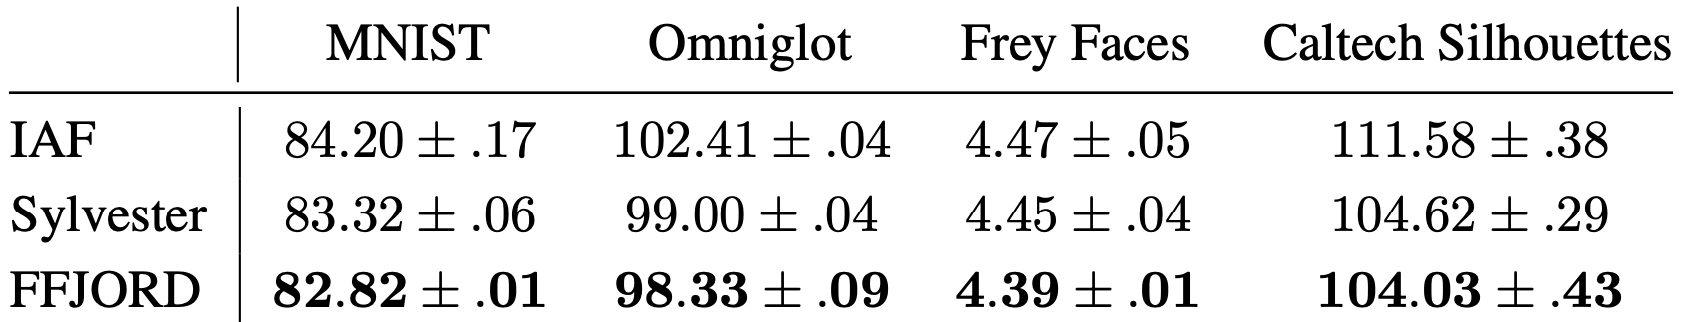
\includegraphics[width=0.8\linewidth]{figs/ffjord_reverse}
		\end{figure}
	\end{block}

	\myfootnotewithlink{https://arxiv.org/abs/1810.01367}{Grathwohl W. et al. FFJORD: Free-form Continuous Dynamics for Scalable Reversible Generative Models, 2018} 
\end{frame}
%=======
\begin{frame}{Discrete VAE}
	\begin{figure}[h]
		\centering
		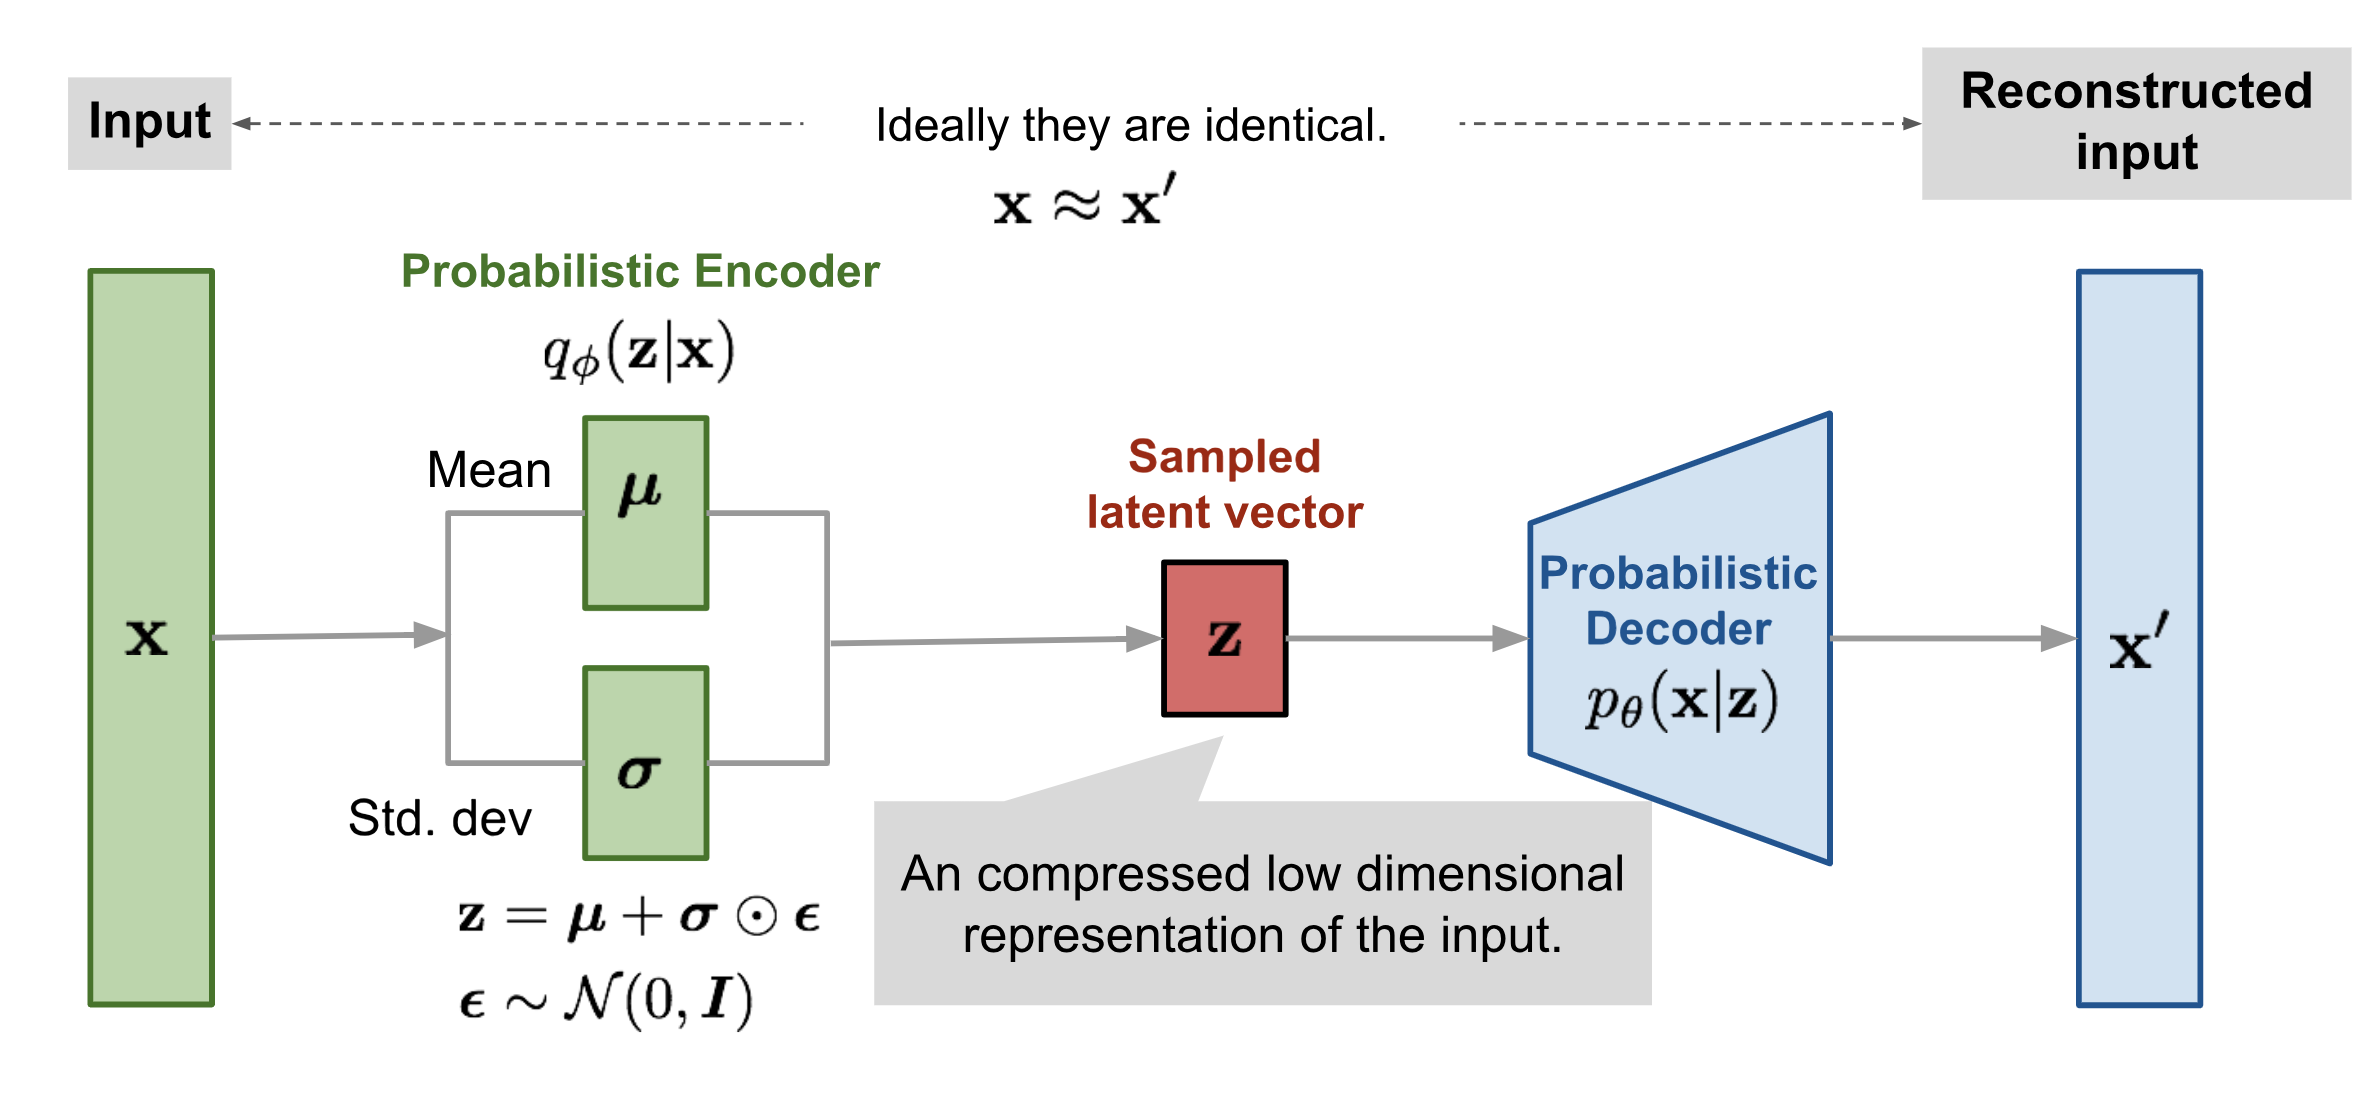
\includegraphics[width=\linewidth]{figs/vae-gaussian.png}
	\end{figure}
	\begin{itemize}
		\item Previous VAE models had \textbf{continuous} latent variables $\bz$.
		\item \textbf{Discrete} representations $\bz$ are potentially a more natural fit for many of the modalities.
		\item Powerful autoregressive models (like PixelCNN) have been developed for modelling distributions over discrete variables.
	\end{itemize}
\end{frame}
%=======
\begin{frame}{Discrete VAE}
	If $\bz$ is a discrete random variable we cannot differentiate through it.
	
	\begin{block}{Gumbel-Max trick}
		Let $G_k \sim \text{Gumbel}$ for $k = 1, \dots, K$, i.e. $G = - \log (\log u)$, $u \sim \text{Uniform}[0, 1]$. Then a discrete random variable
		\vspace{-0.2cm}
		\[
			z = \argmax_k (\log \pi_k + G_k), \quad \sum_k \pi_k = 1
		\]
		\vspace{-0.5cm} \\
		has a categorical distribution $z \sim \text{Categorical}(\bpi)$ ($P(z = k) = \pi_k$).
	\end{block}
	\textbf{Problem:} We still have non-differentiable $\argmax$ operation.
	\begin{block}{Gumbel-Softmax relaxation}
		
		\[
			z_k = \frac{\exp ((\log \pi_k + G_k) / \tau)}{\sum_{j=1}^K \exp ((\log \pi_j + G_j) / \tau)}, \quad k = 1, \dots, K.
		\]
		Here $\tau$ is a temperature parameter.
 	\end{block}
	\myfootnote{
	\href{https://arxiv.org/abs/1611.00712}{Maddison C. J., Mnih A., Teh Y. W. The Concrete distribution: A continuous relaxation of discrete random variables, 2016} \\
	\href{https://arxiv.org/abs/1611.01144}{Jang E., Gu S., Poole B. Categorical reparameterization with Gumbel-Softmax, 2016}
	}
\end{frame}%=======
\begin{frame}{Discrete VAE}
	\vspace{-0.3cm}
	\begin{block}{Gumbel-Softmax relaxation}
		Concrete distribution = continuous + discrete
		\vspace{-0.2cm}
		\[
			z_k = \frac{\exp ((\log \pi_k + G_k) / \tau)}{\sum_{j=1}^K \exp ((\log \pi_j + G_j) / \tau)}, \quad k = 1, \dots, K.
		\]
		\vspace{-0.4cm} \\
		Here $\tau$ is a temperature parameter. Now we have differentiable operation.
 	\end{block}
 	\vspace{-0.2cm}
 	\begin{figure}
 		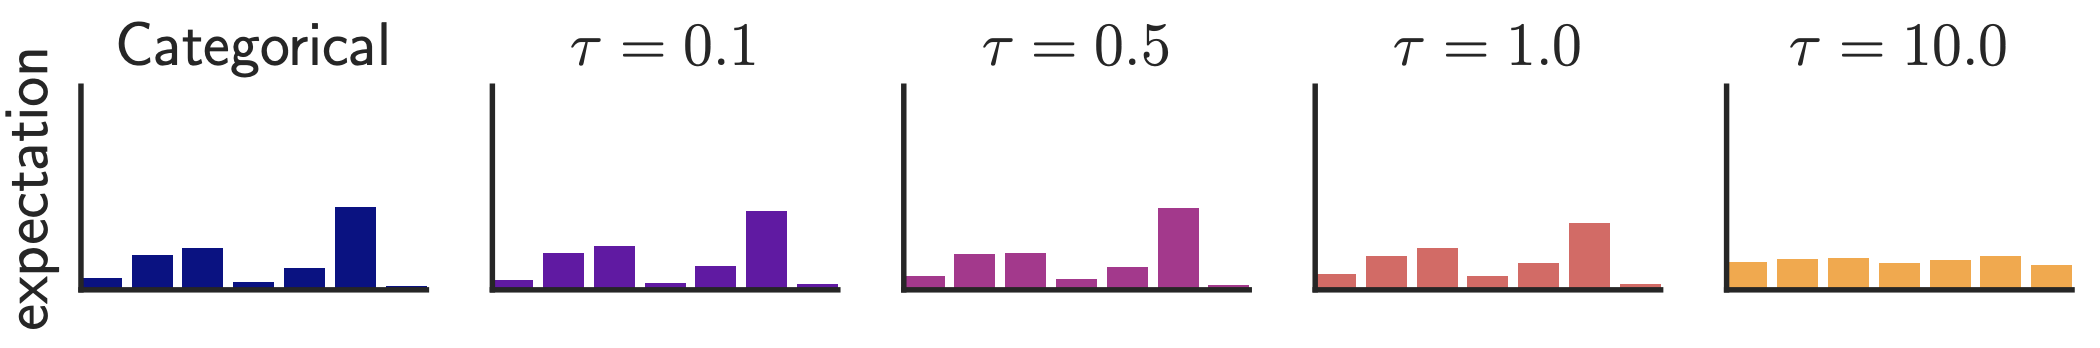
\includegraphics[width=0.8\linewidth]{figs/gumbel_softmax}
 	\end{figure}
 	\vspace{-0.7cm}
 	\begin{figure}
 		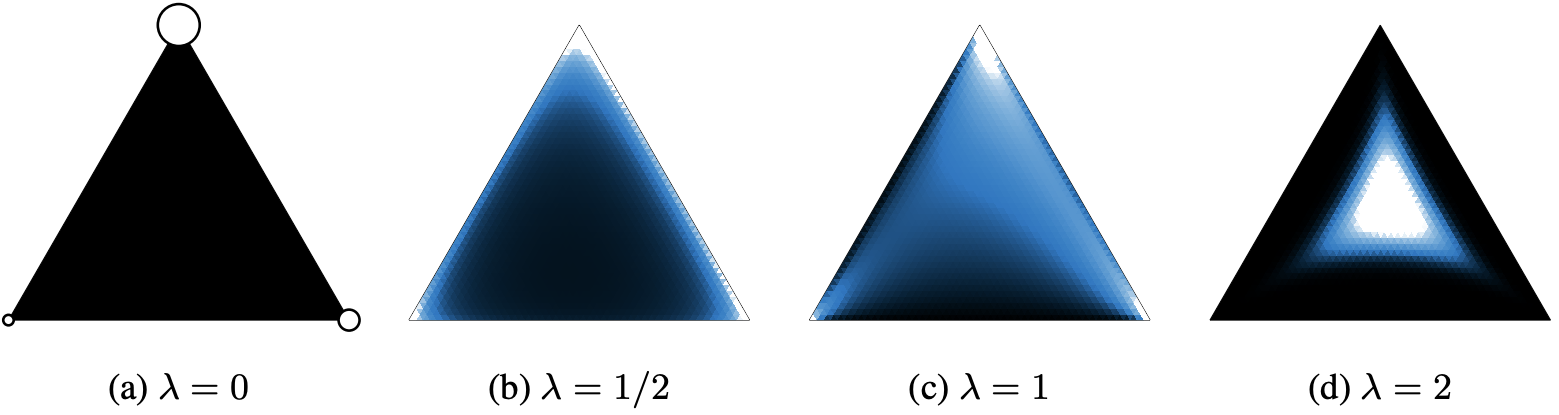
\includegraphics[width=0.8\linewidth]{figs/simplex}
 	\end{figure} 
	\myfootnote{
	\href{https://arxiv.org/abs/1611.00712}{Maddison C. J., Mnih A., Teh Y. W. The Concrete distribution: A continuous relaxation of discrete random variables, 2016} \\
	\href{https://arxiv.org/abs/1611.01144}{Jang E., Gu S., Poole B. Categorical reparameterization with Gumbel-Softmax, 2016}
	}
\end{frame}
%=======
\begin{frame}{Vector Quantized VAE}
	\begin{itemize}
		\item Define dictionary space $\{\be_k\}_{k=1}^K$, where $\be_k \in \bbR^C$, $K$ is the size of the dictionary.
		\item Let $\bz = \text{NN}_\text{e}(\bx) \in \bbR^{W \times H \times C}$ be an encoder output.
		\item Quantized representation $\bz_q \in \bbR^{W \times H \times C}$ is defined by a nearest neighbour look-up using the shared dictionary space for each of $W \times H$ spatial locations
		\vspace{-0.2cm}
		\[
			[\bz_q]_{ij} = \be_{k^*}, \quad \text{where } k^* = \argmin_k \| [\bz_e]_{ij} - \be_k \|.
		\] 
	\end{itemize}
	\vspace{-0.6cm}
	\begin{block}{Quantization procedure}
		\begin{minipage}[t]{0.65\columnwidth}
			\begin{figure}
				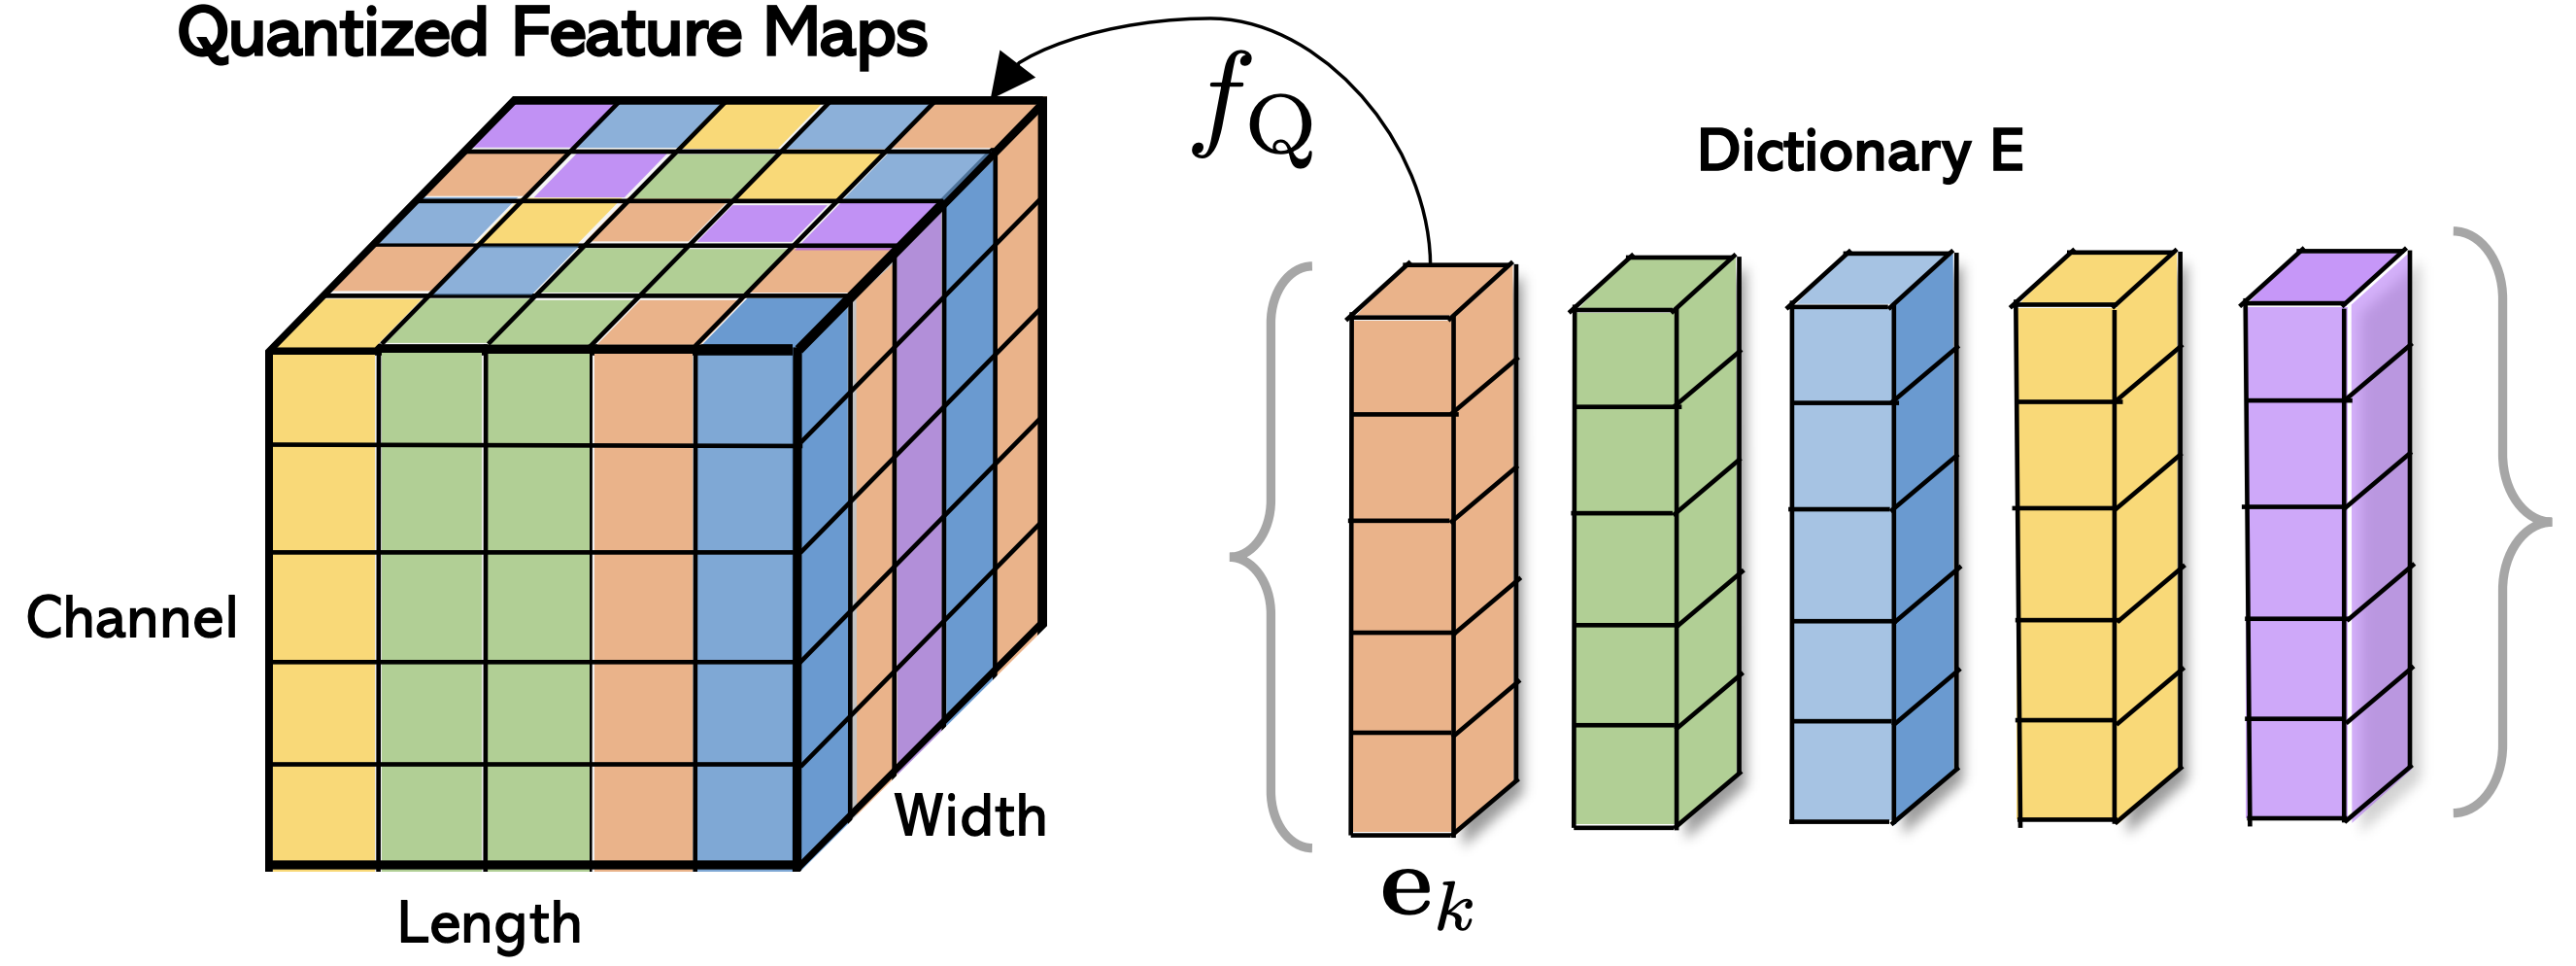
\includegraphics[width=\linewidth]{figs/fqgan_cnn.png}
			\end{figure}
		\end{minipage}%
		\begin{minipage}[t]{0.35\columnwidth}
			\begin{figure}
				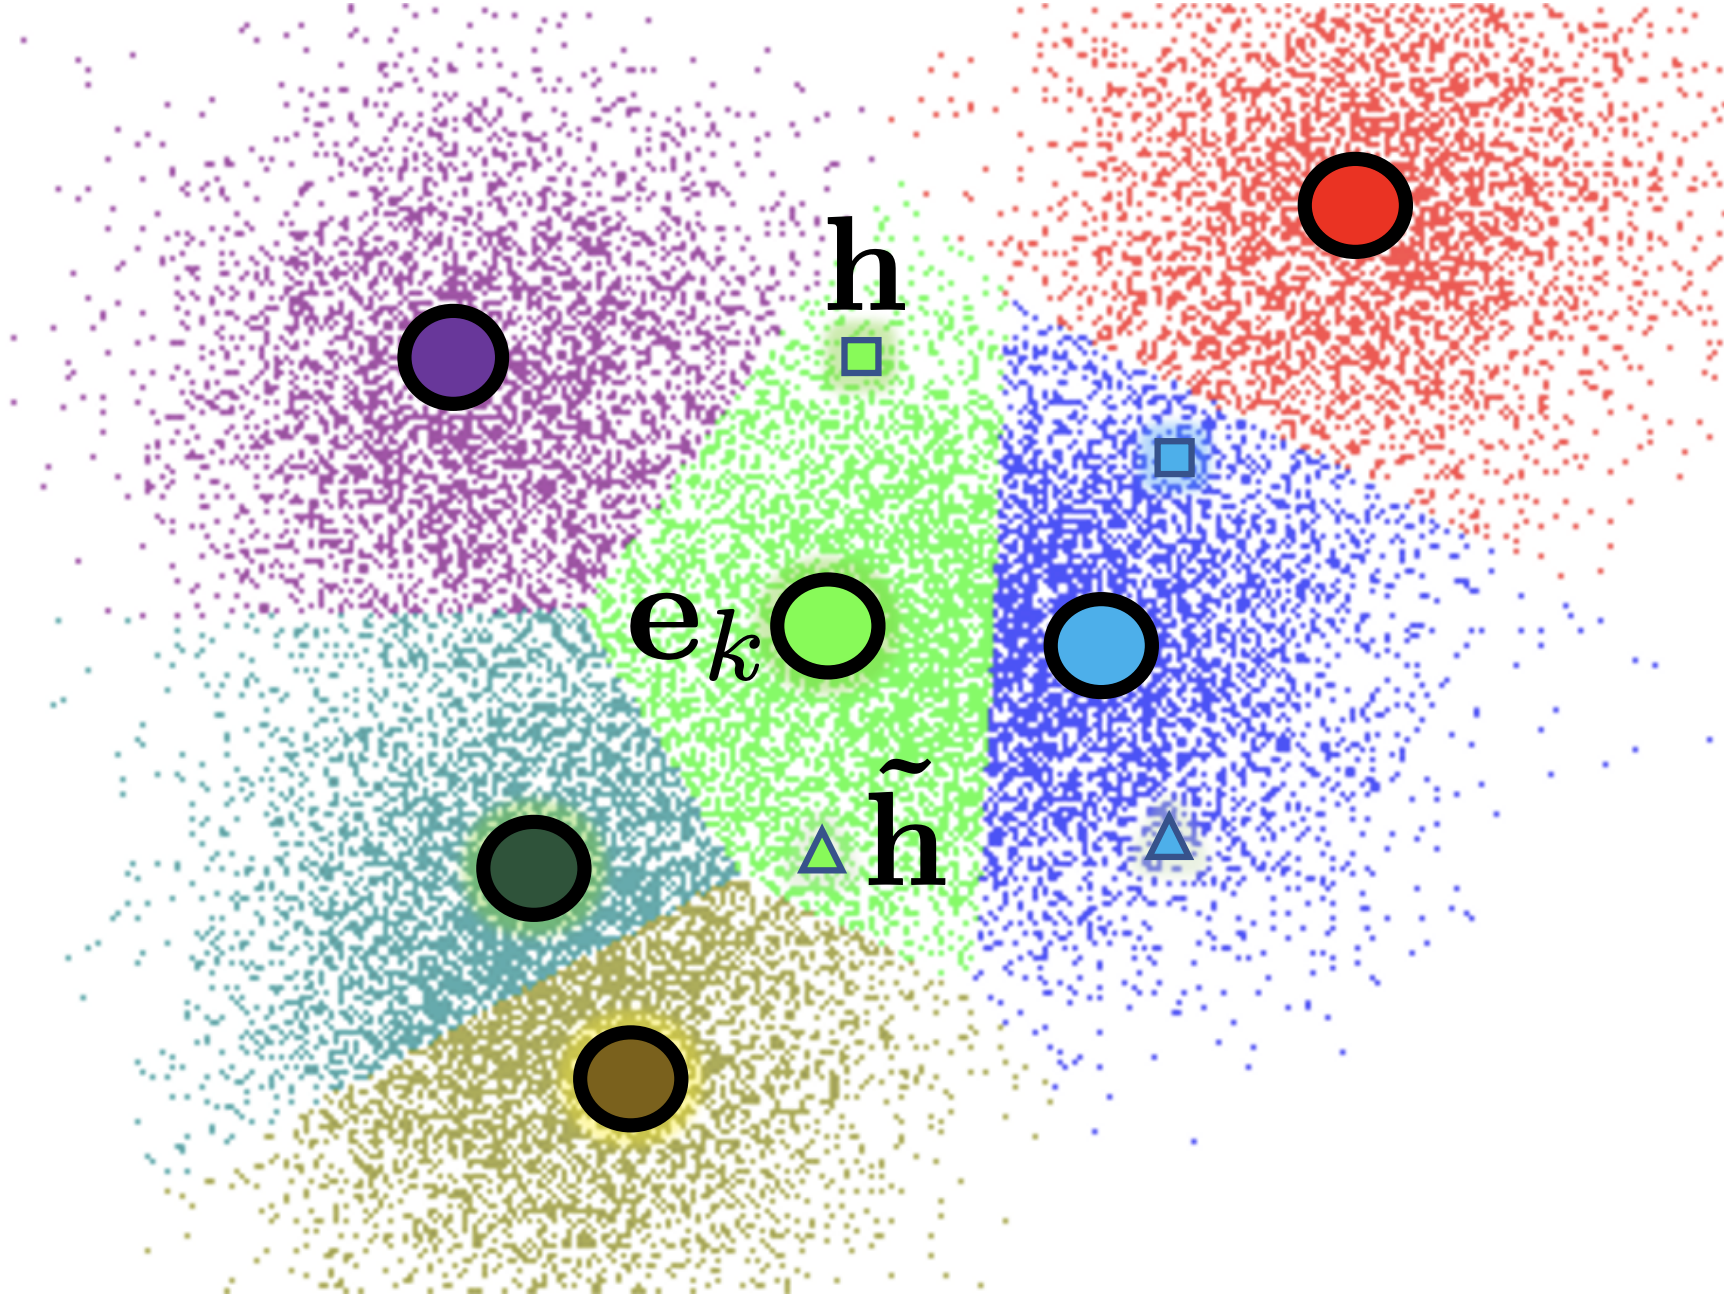
\includegraphics[width=0.9\linewidth]{figs/fqgan_lookup}
			\end{figure}
		\end{minipage}
	\end{block}

	\myfootnotewithlink{https://arxiv.org/abs/2004.02088}{Zhao Y. et al. Feature Quantization Improves GAN Training, 2020} 
\end{frame}
%=======
\begin{frame}{Vector Quantized VAE}
	Define VAE latent variable $\hat{\bz} \in \bbR^{W \times H}$ with prior distribution $p(\hat{\bz}) = \text{Uniform}\{1, \dots, K\}$ and variational posterior distribution 
	\vspace{-0.3cm}
	\[
		q(\hat{\bz} | \bx) = \prod_{i=1}^W \prod_{j=1}^H q(\hat{z}_{ij} | \bx)
	\]
	\vspace{-0.3cm}
	\[
		q(\hat{z}_{ij} = k^* | \bx) = \begin{cases}
			1 , \quad \text{for } k^* = \argmin_k \| [\bz_e]_{ij} - \be_k \| \\
			0, \quad \text{otherwise}.
		\end{cases}
	\]
	\vspace{-0.5cm}
	\begin{block}{ELBO objective}
		\vspace{-0.5cm}
		\[
		 \mathcal{L} (\bphi, \btheta)  = \mathbb{E}_{q(\hat{\bz} | \bx, \bphi)} \log p(\bx | \hat{\bz}, \btheta)] - KL(q(\hat{\bz}| \bx) || p(\hat{\bz})) \rightarrow \max_{\bphi, \btheta}.
		\]	
		\vspace{-0.5cm}
	\end{block}
	\begin{itemize}
		\item VAE proposal distribution $q(\hat{\bz} | \bx)$ is deterministic. 
		\item $KL(q(\hat{z}| \bx) || p(\hat{z}))$ term in ELBO is constant (equals to $\log K$).
	\end{itemize}
	
	\myfootnotewithlink{https://arxiv.org/abs/1711.00937}{Oord A., Vinyals O., Kavukcuoglu K. Neural Discrete Representation Learning, 2017} 
\end{frame}
%=======
\begin{frame}{Vector Quantized VAE}
	\begin{figure}
		\centering
		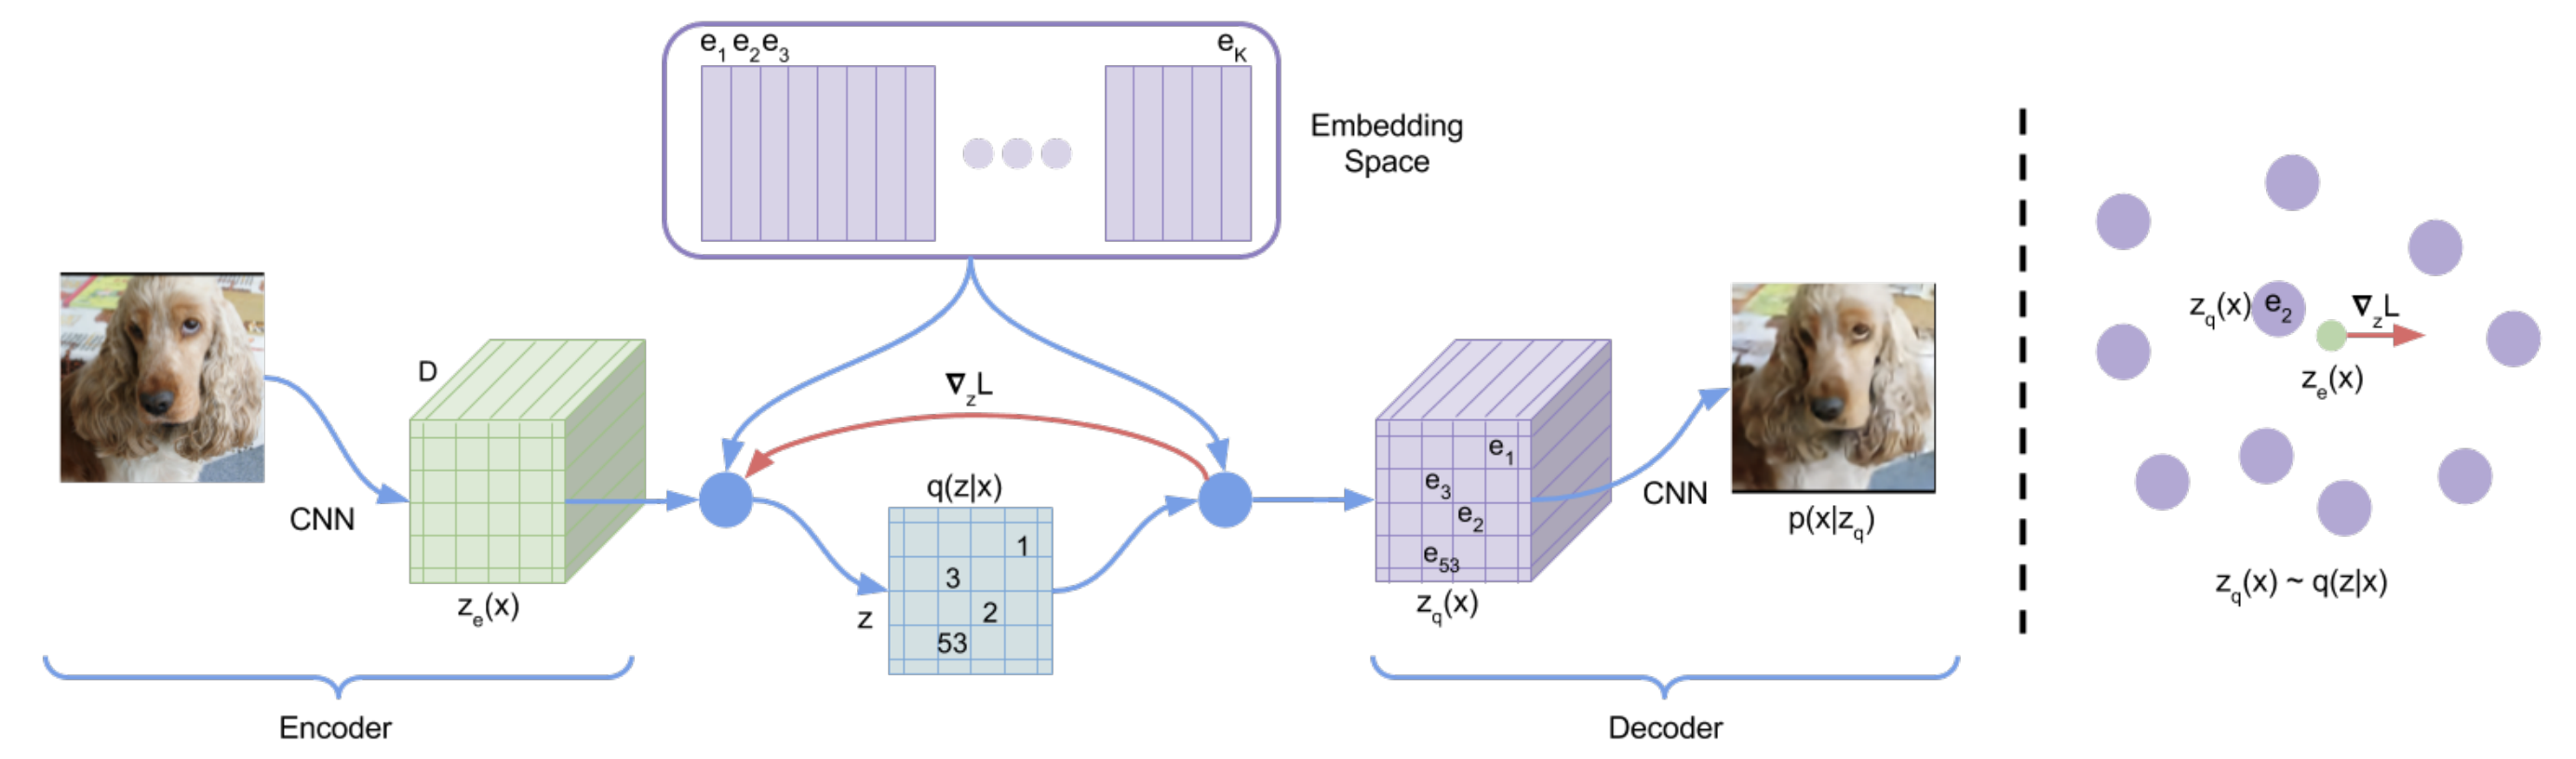
\includegraphics[width=\linewidth]{figs/vqvae}
	\end{figure}
	\begin{block}{Objective}
		\vspace{-0.3cm}
		\[
			\log p(\bx | \bz_q) + \| \text{sg} (\bz_e) - \bz_q \| + \beta \| \bz_e - \text{sg}(\bz_q) \|
		\]
	\end{block}
	\begin{itemize}
		\item First term is ELBO part.
		\item Quantization operation is not differentiable.
		\item Straight-through gradient estimation is used to backpropagate the quantization operation.
	\end{itemize}

	\myfootnotewithlink{https://arxiv.org/abs/1711.00937}{Oord A., Vinyals O., Kavukcuoglu K. Neural Discrete Representation Learning, 2017} 
\end{frame}
%=======
\begin{frame}{Vector Quantized VAE-2}
	\begin{block}{Samples 1024x1024}
		\vspace{-0.2cm}
		\begin{figure}
			\centering
			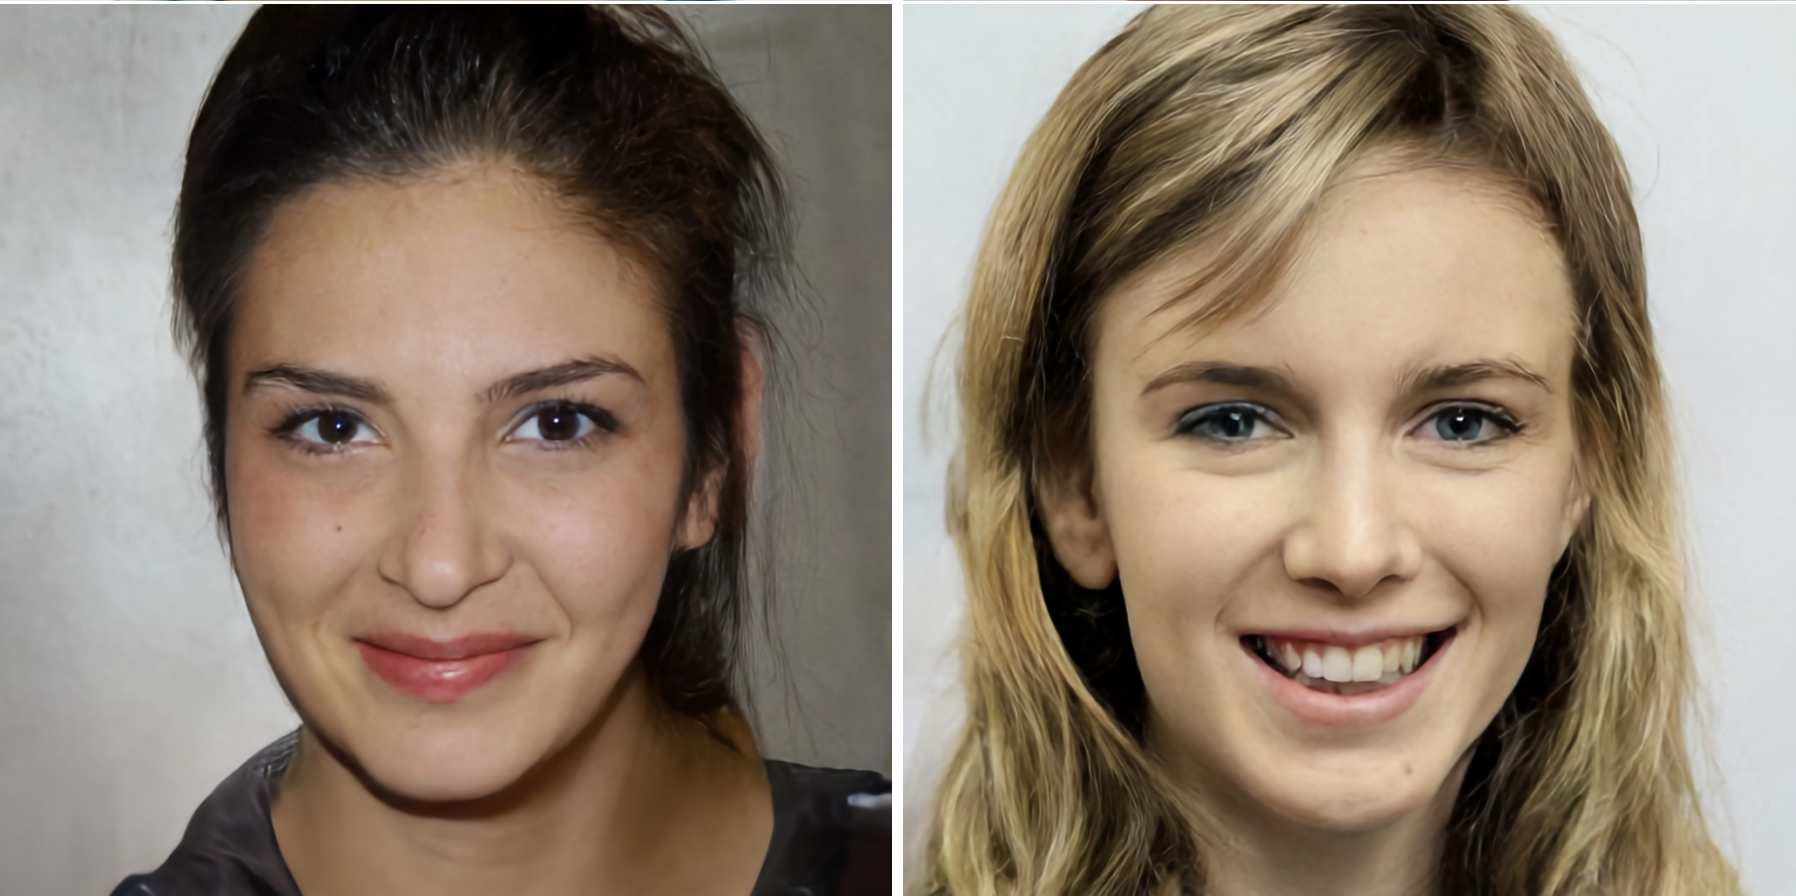
\includegraphics[width=0.63\linewidth]{figs/vqvae2_faces}
		\end{figure}
	\end{block}
	\vspace{-0.6cm}
	\begin{block}{Samples diversity}
		\vspace{-0.2cm}
		\begin{figure}
			\centering
			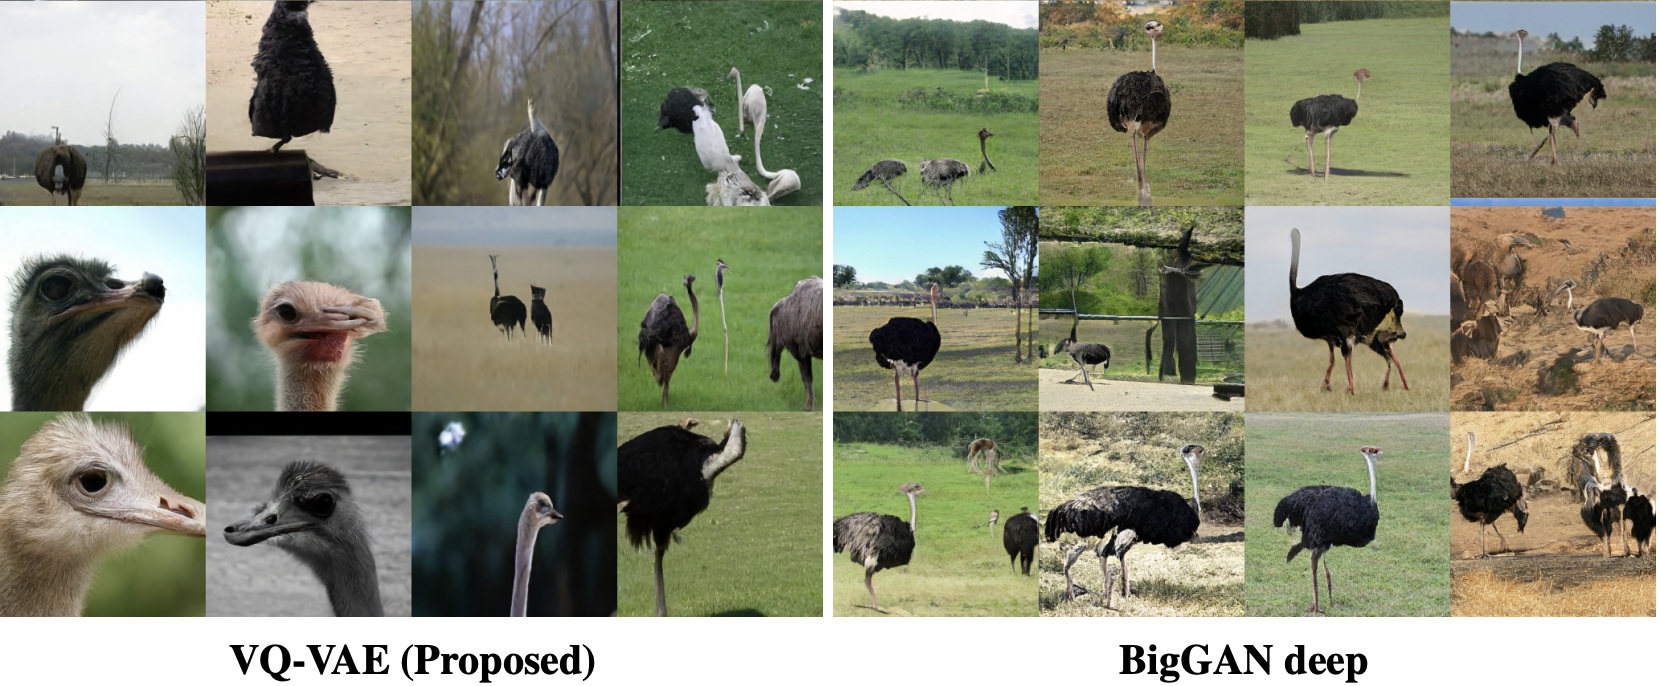
\includegraphics[width=0.65\linewidth]{figs/vqvae2_diversity}
		\end{figure}
	\end{block}
	\myfootnotewithlink{https://arxiv.org/abs/1906.00446}{Razavi A., Oord A., Vinyals O. Generating Diverse High-Fidelity Images with VQ-VAE-2, 2019} 
\end{frame}
%=======
\begin{frame}{DALL-E}
	\begin{block}{Deterministic VQ-VAE posterior}
		\vspace{-0.3cm}
		\[
			q(\hat{z}_{ij} = k^* | \bx) = \begin{cases}
				1 , \quad \text{for } k^* = \argmin_k \| [\bz_e]_{ij} - \be_k \| \\
				0, \quad \text{otherwise}.
			\end{cases}
		\]
		\vspace{-0.3cm}
	\end{block}
	\begin{itemize}
		\item It is possible to use Gumbel-Softmax trick to relax this distribution to continuous one.
		\item Since latent space is discrete we could train autoregressive transformers in it.
		\item It is a natural way to incorporate text and image spaces.
	\end{itemize}
	\begin{figure}
		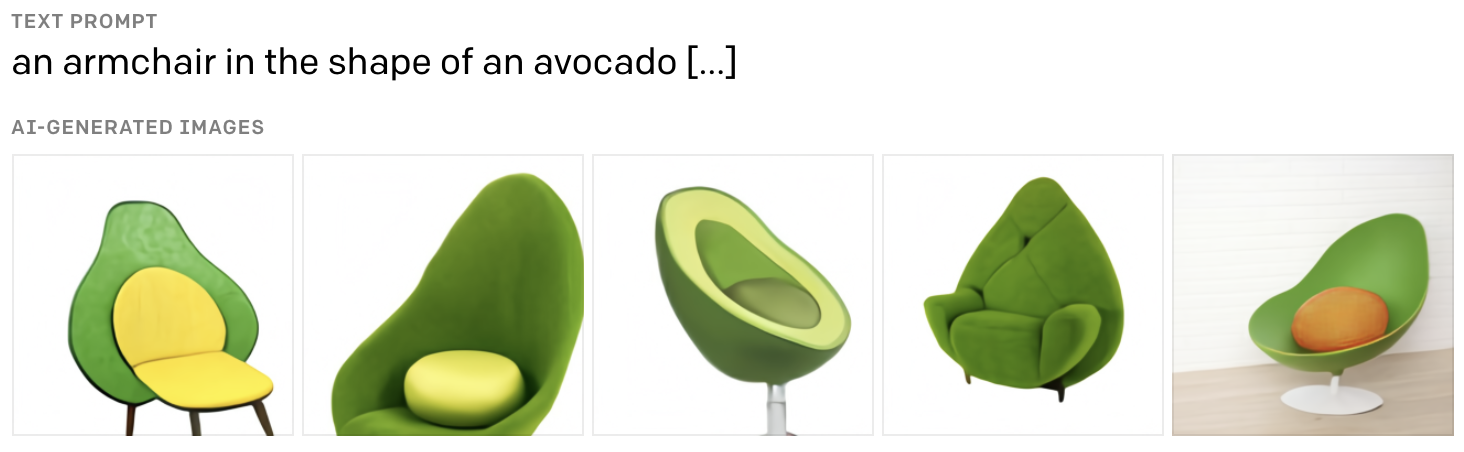
\includegraphics[width=\linewidth]{figs/dalle}
	\end{figure}
	\myfootnotewithlink{https://arxiv.org/abs/2102.1209}{Ramesh A. et al. Zero-shot text-to-image generation, 2021}
\end{frame}
%=======
\begin{frame}{Summary}
	\begin{itemize}
	\item Residual networks could be interpreted as solution of ODE with Euler method.
	\vfill
	\item Adjoint method generalizes backpropagation procedure and allows to train Neural ODE solving ODE for adjoint function back in time.
	\vfill
	\item Fokker-Planck theorem allows to construct continuous-in-time normalizing flow with less functional restrictions.
	\vfill
	\item FFJORD model makes such kind of flows scalable.
	\vfill
	\item Gumbel-Softmax and Quantization are the two ways to create VAE with discrete latent space.
	\vfill
	\item It becomes more and more popular to use discrete latent spaces in the fields of image/video/music generaton.
	\end{itemize}
\end{frame}
\end{document} 